\section{Graphical User Interface}

This section contains a beta version of the system's graphical user interface (GUI).

When the user opens the GUI, the main window, shown in figure~\ref{fig:mainWindow}, appears. The user needs to select a sphere in order to proceed.  Figure~\ref{fig:viewSphere} shows how the window looks when a sphere is selected. When the user selects retrieval mode, the right part of the GUI changes. Figure~\ref{fig:retrievalMode} shows how the window looks at this moment.  When the user selects one of the download options the GUI asks for the location where the user wants to store the data, as shown in figure~\ref{fig:download}. When the user selects sampling mode, a progress bar will appear for the duration of the sample. Figure~\ref{fig:samplingMode} shows how the window looks in this mode. After the sampling time has passed, the GUI automatically enters in locate mode and opens a pop-up to show location information, as shown in figure~\ref{fig:locateMode}. When the user selects diagnostic mode, a pop-up showing diagnosic information appears, as shown in figure~\ref{fig:diagnosticMode}.

\begin{figure}[H]
	\centering
	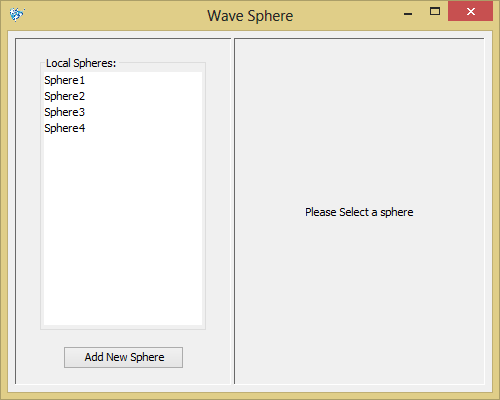
\includegraphics[scale=0.7]{img/mainWindow}
	\caption{Main Window \label{fig:mainWindow}}
\end{figure}

\begin{figure}[H]
	\centering
	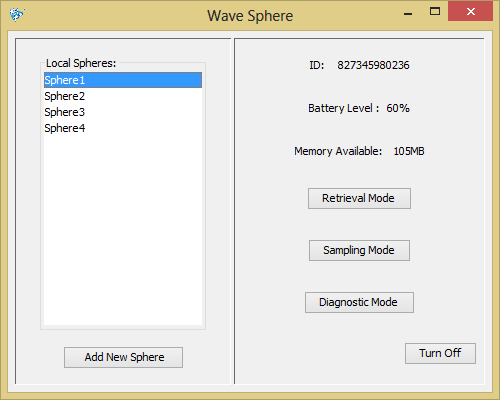
\includegraphics[scale=0.7]{img/viewSphere}
	\caption{Sphere View \label{fig:viewSphere}}
\end{figure}

\begin{figure}[H]
	\centering
	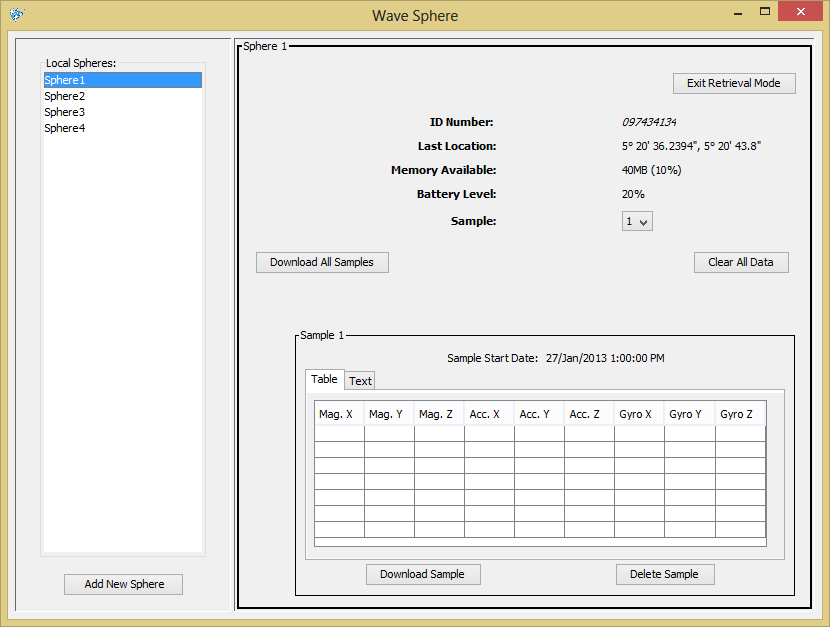
\includegraphics[scale=0.7]{img/retrievalMode}
	\caption{Retrieval Mode \label{fig:retrievalMode}}
\end{figure}

\begin{figure}[H]
	\centering
	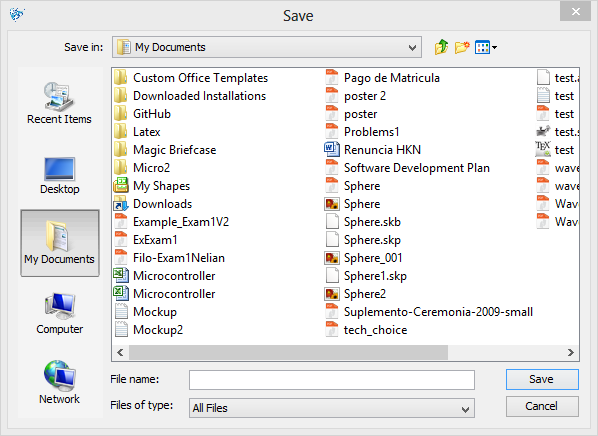
\includegraphics[scale=0.7]{img/download}
	\caption{Download \label{fig:download}}
\end{figure}

\begin{figure}[H]
	\centering
	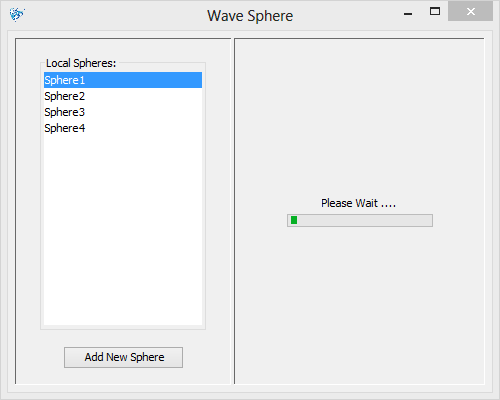
\includegraphics[scale=0.7]{img/samplingMode}
	\caption{Sampling Mode \label{fig:samplingMode}}
\end{figure}

\begin{figure}[H]
	\centering
	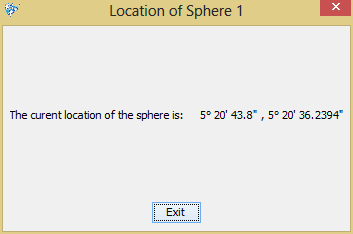
\includegraphics[scale=0.7]{img/locateMode}
	\caption{Locate Mode \label{fig:locateMode}}
\end{figure}

\begin{figure}[H]
	\centering
	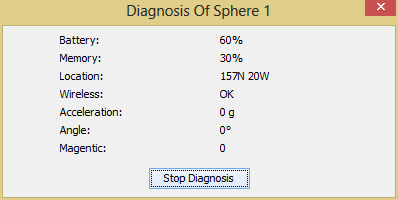
\includegraphics[scale=0.7]{img/diagnosticMode}
	\caption{Diagnostic Mode \label{fig:diagnosticMode}}
\end{figure}